


\subsubsection{Training Loop}
\label{sec:Method:Learning:TrainingLoop}
The training loop for the proposed model is presented in the algorithm below:

\begin{algorithm}[H] 
\caption{Training of the Stepwise Constant Velocity Model. Return the log-likelihood of events.}
\label{alg:TrainingLoop}
\begin{algorithmic}%[1]
\Require{Batch of entire dataset of event tuples $(u_i, v_i, t_i)$, for $i = 1,\dots,n$. Also number of velocities, steps $s = 1,\dots,m$, to fit.} 
\Ensure{log-likelihood $\ell$}
\Statex

\State {$EventIntensity = 0$}
\State {$NonEventIntensity = 0$}

\For{m}                    
    \State {$EventIntensity_s = 0$}
    \For{$u_{s,i}, v_{s,i}, t_{s,i}$} 
        \State {$EventIntensity_s \mathrel{+}= \beta - ||z_u(t) - \z_v(t)||_2^2$}
    \EndFor
    \State {$EventIntensity \mathrel{+}= EventIntensity_s$}
\EndFor
\\
\For{m} 
    \State {$NonEventIntensity_s = 0$}
    \For{$NodePair: u,v$} 
        \State {$NonEventIntensity_s \mathrel{+}= integral(u, v, t_0, t_n, n)$}
    \EndFor
    \State {$NonEventIntensity \mathrel{+}= NonEventIntensity_s$}
\EndFor
\\
\State {$LogLikelihood = - EventIntensity - NonEventIntensity$}
\State \Return {$LogLikelihood$}
\EndFunction
\end{algorithmic}
\end{algorithm}
NOT COMPLETELY FINISHED, BUT THE FINAL PART OF THIS SECTION NONTHELESS.









\begin{figure}[H]
    \centering
    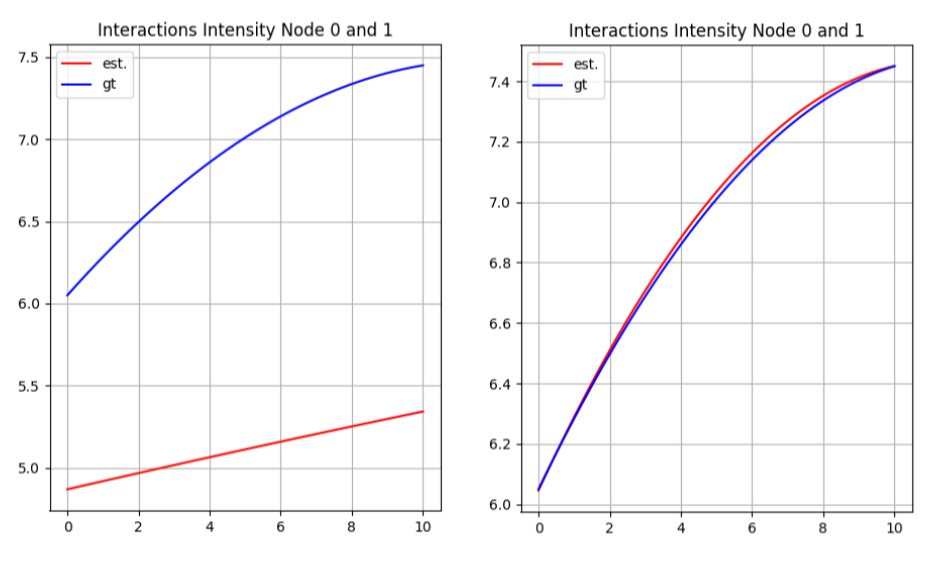
\includegraphics[width=\textwidth]{0_images/5vs5000epochs.png}
    \caption{Example of Interaction Intensity Comparison: Interaction intensity (y-axis) from time 0 to 10 (x-axis) between nodes 0 and 1 for a given system. Blue is the ground truth model and red is the trained model. Left compares intensities after training the model for 5 epochs, right after training for 5000 epochs.}
    \label{fig:5vs5000epochs}
\end{figure}






\subsubsection{Squared Euclidean Distance}
\label{sec:Method:LSM:SquaredEuclideanDistance}
The reciprocal distances between nodes are calculated as the squared Euclidean distance, which is expressed below, very similar to the standard Euclidean distance:

\begin{align} 
||\textbf{z}_u(t) - \textbf{z}_v(t)||_2^2
&= 
\left(\sqrt{((x_u + v_{x,u}t) - (x_v + v_{x,v}t))^2 + ((y_u + v_{y,u}t) - (y_v + v_{y,v}t))^2}\right)^2
\\
&=
((x_u + v_{x,u}t) - (x_v + v_{x,v}t))^2 + ((y_u + v_{y,u}t) - (y_v + v_{y,v}t))^2
\\
&=
(x_u - x_v + (v_{x,u} - v_{x,v})t)^2 + (y_u - y_v + ( v_{y,u} - v_{y,v})t)^2
\end{align}




% \subsubsection{Bias Term $\beta$}
% \label{sec:Method:IntensityFunc:BiasTerm}

% The bias term, $\beta$, a part of the intensity function, is a learnable parameter for the model.
% This project considers two different implementations of the bias term. One version uses a \textit{common bias term} with a single $\beta$ scalar parameter as explained for equation (\ref{eq:IntensityFunc}) above.
% An alternative to the common bias term is the \textit{node specific bias term} where a bias term is added for each node $i$, such that the scalar $\beta_i$ is a learnable model parameter for the bias of node $i$. This results in a model with a learnable parameter vector $\beta \in \mathbb{R}^N$ where $N$ is the number of nodes in the network. Then the intensity function is written as:
% \begin{equation}
%         \lambda_{u,v}(t)
%     =
%     \exp \left(\beta_u + \beta_v - ||\textbf{z}_u(t) - \textbf{z}_v(t)||_2^2\right)
%     \label{eq:NodeBiasIntensityFunc}
% \end{equation}

% For this report the common bias term model will be the primary implementation of consideration.






\subsubsection{152 node synthetic dataset}
\label{sec:ResearchQuestion2:150nodeSynthetic}

Synthetic dataset 3, see section \ref{sec:Data:SyntheticData:SyntheticDataset3}, is utilized here.
\\\\
\textbf{Loss and beta convergence results.}

\begin{table}[h!]
\centering
\begin{tabular}{|l|cc|}
\hline
Batch Size   & Beta & NLL\\ \hline
Ground Truth & 7.5  & 79,424      \\
50,000          & XX   & XX       \\
Full          & XX   & XX       \\
\hline
\end{tabular}
\caption{}
\label{tab:SingleStep1}
\end{table}
\noindent \textbf{Intensity rate comparison results.}
\\\\
\textbf{Animation check.}
\\\\
\textbf{Dyad removal results.}
\\\\
\textbf{Interaction removal results.}
   



\subsubsection{986 node real dataset}
\label{sec:ResearchQuestion2:986nodeReal}

Real dataset 2, see section \ref{sec:Data:RealData:RealDataset2}, is utilized here.
\\\\
\textbf{Animation check.}
\\\\
\textbf{Diad removal results.}
\\\\
\textbf{Interaction removal results.}

